\documentclass[tikz,border=8pt]{standalone}
\usepackage[utf8]{inputenc}
\usepackage{amsmath,amssymb}
\usepackage{csquotes}
\usetikzlibrary{arrows.meta, positioning, calc}
\renewcommand{\familydefault}{\sfdefault}
\begin{document}
	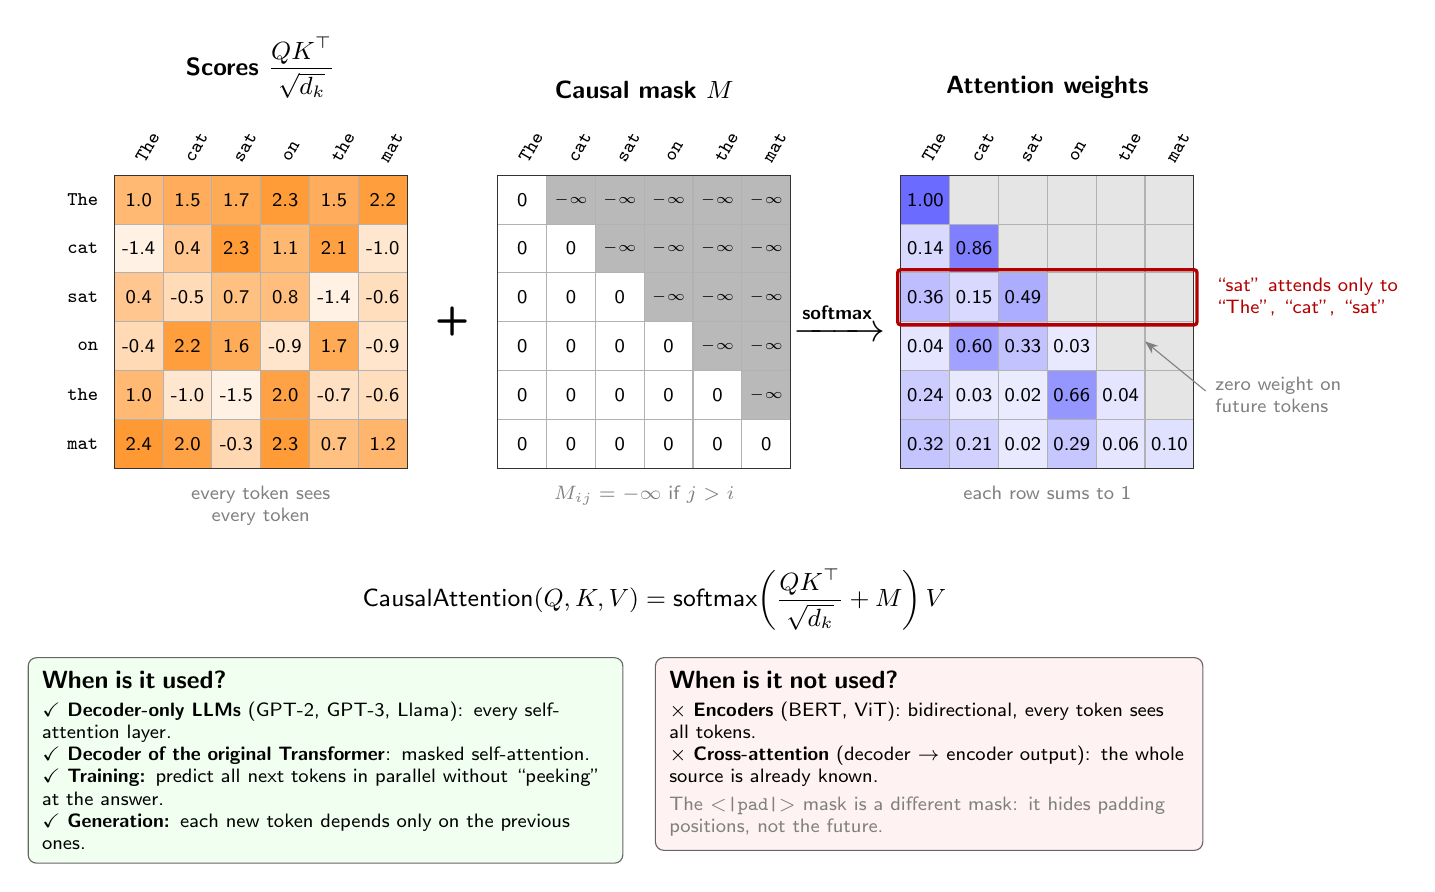
\begin{tikzpicture}[
		ttl/.style={font=\sffamily\small\bfseries, anchor=south, align=center},
		sub/.style={font=\sffamily\scriptsize, text=gray, anchor=north, align=center},
		op/.style={font=\sffamily\Large\bfseries},
		cellv/.style={font=\sffamily\scriptsize}
		]
		\fill[orange!55!white] (0.00,0.00) rectangle ++(0.62,-0.62);
		\node[cellv] at (0.31,-0.31) {1.0};
		\fill[orange!64!white] (0.62,0.00) rectangle ++(0.62,-0.62);
		\node[cellv] at (0.93,-0.31) {1.5};
		\fill[orange!67!white] (1.24,0.00) rectangle ++(0.62,-0.62);
		\node[cellv] at (1.55,-0.31) {1.7};
		\fill[orange!78!white] (1.86,0.00) rectangle ++(0.62,-0.62);
		\node[cellv] at (2.17,-0.31) {2.3};
		\fill[orange!64!white] (2.48,0.00) rectangle ++(0.62,-0.62);
		\node[cellv] at (2.79,-0.31) {1.5};
		\fill[orange!76!white] (3.10,0.00) rectangle ++(0.62,-0.62);
		\node[cellv] at (3.41,-0.31) {2.2};
		\fill[orange!11!white] (0.00,-0.62) rectangle ++(0.62,-0.62);
		\node[cellv] at (0.31,-0.93) {-1.4};
		\fill[orange!44!white] (0.62,-0.62) rectangle ++(0.62,-0.62);
		\node[cellv] at (0.93,-0.93) {0.4};
		\fill[orange!78!white] (1.24,-0.62) rectangle ++(0.62,-0.62);
		\node[cellv] at (1.55,-0.93) {2.3};
		\fill[orange!56!white] (1.86,-0.62) rectangle ++(0.62,-0.62);
		\node[cellv] at (2.17,-0.93) {1.1};
		\fill[orange!74!white] (2.48,-0.62) rectangle ++(0.62,-0.62);
		\node[cellv] at (2.79,-0.93) {2.1};
		\fill[orange!19!white] (3.10,-0.62) rectangle ++(0.62,-0.62);
		\node[cellv] at (3.41,-0.93) {-1.0};
		\fill[orange!44!white] (0.00,-1.24) rectangle ++(0.62,-0.62);
		\node[cellv] at (0.31,-1.55) {0.4};
		\fill[orange!28!white] (0.62,-1.24) rectangle ++(0.62,-0.62);
		\node[cellv] at (0.93,-1.55) {-0.5};
		\fill[orange!49!white] (1.24,-1.24) rectangle ++(0.62,-0.62);
		\node[cellv] at (1.55,-1.55) {0.7};
		\fill[orange!51!white] (1.86,-1.24) rectangle ++(0.62,-0.62);
		\node[cellv] at (2.17,-1.55) {0.8};
		\fill[orange!11!white] (2.48,-1.24) rectangle ++(0.62,-0.62);
		\node[cellv] at (2.79,-1.55) {-1.4};
		\fill[orange!26!white] (3.10,-1.24) rectangle ++(0.62,-0.62);
		\node[cellv] at (3.41,-1.55) {-0.6};
		\fill[orange!29!white] (0.00,-1.86) rectangle ++(0.62,-0.62);
		\node[cellv] at (0.31,-2.17) {-0.4};
		\fill[orange!76!white] (0.62,-1.86) rectangle ++(0.62,-0.62);
		\node[cellv] at (0.93,-2.17) {2.2};
		\fill[orange!65!white] (1.24,-1.86) rectangle ++(0.62,-0.62);
		\node[cellv] at (1.55,-2.17) {1.6};
		\fill[orange!20!white] (1.86,-1.86) rectangle ++(0.62,-0.62);
		\node[cellv] at (2.17,-2.17) {-0.9};
		\fill[orange!67!white] (2.48,-1.86) rectangle ++(0.62,-0.62);
		\node[cellv] at (2.79,-2.17) {1.7};
		\fill[orange!20!white] (3.10,-1.86) rectangle ++(0.62,-0.62);
		\node[cellv] at (3.41,-2.17) {-0.9};
		\fill[orange!55!white] (0.00,-2.48) rectangle ++(0.62,-0.62);
		\node[cellv] at (0.31,-2.79) {1.0};
		\fill[orange!19!white] (0.62,-2.48) rectangle ++(0.62,-0.62);
		\node[cellv] at (0.93,-2.79) {-1.0};
		\fill[orange!10!white] (1.24,-2.48) rectangle ++(0.62,-0.62);
		\node[cellv] at (1.55,-2.79) {-1.5};
		\fill[orange!73!white] (1.86,-2.48) rectangle ++(0.62,-0.62);
		\node[cellv] at (2.17,-2.79) {2.0};
		\fill[orange!24!white] (2.48,-2.48) rectangle ++(0.62,-0.62);
		\node[cellv] at (2.79,-2.79) {-0.7};
		\fill[orange!26!white] (3.10,-2.48) rectangle ++(0.62,-0.62);
		\node[cellv] at (3.41,-2.79) {-0.6};
		\fill[orange!80!white] (0.00,-3.10) rectangle ++(0.62,-0.62);
		\node[cellv] at (0.31,-3.41) {2.4};
		\fill[orange!73!white] (0.62,-3.10) rectangle ++(0.62,-0.62);
		\node[cellv] at (0.93,-3.41) {2.0};
		\fill[orange!31!white] (1.24,-3.10) rectangle ++(0.62,-0.62);
		\node[cellv] at (1.55,-3.41) {-0.3};
		\fill[orange!78!white] (1.86,-3.10) rectangle ++(0.62,-0.62);
		\node[cellv] at (2.17,-3.41) {2.3};
		\fill[orange!49!white] (2.48,-3.10) rectangle ++(0.62,-0.62);
		\node[cellv] at (2.79,-3.41) {0.7};
		\fill[orange!58!white] (3.10,-3.10) rectangle ++(0.62,-0.62);
		\node[cellv] at (3.41,-3.41) {1.2};
		\draw[step=0.62, black!30, xshift=0cm] (0,0) grid (3.72,-3.72);
		\draw[black!80] (0,0) rectangle ++(3.72,-3.72);
		\node[font=\ttfamily\scriptsize, rotate=60, anchor=west] at (0.26,0.08) {The};
		\node[font=\ttfamily\scriptsize, rotate=60, anchor=west] at (0.88,0.08) {cat};
		\node[font=\ttfamily\scriptsize, rotate=60, anchor=west] at (1.50,0.08) {sat};
		\node[font=\ttfamily\scriptsize, rotate=60, anchor=west] at (2.12,0.08) {on};
		\node[font=\ttfamily\scriptsize, rotate=60, anchor=west] at (2.74,0.08) {the};
		\node[font=\ttfamily\scriptsize, rotate=60, anchor=west] at (3.36,0.08) {mat};
		\node[font=\ttfamily\scriptsize, anchor=east] at (-0.08,-0.31) {The};
		\node[font=\ttfamily\scriptsize, anchor=east] at (-0.08,-0.93) {cat};
		\node[font=\ttfamily\scriptsize, anchor=east] at (-0.08,-1.55) {sat};
		\node[font=\ttfamily\scriptsize, anchor=east] at (-0.08,-2.17) {on};
		\node[font=\ttfamily\scriptsize, anchor=east] at (-0.08,-2.79) {the};
		\node[font=\ttfamily\scriptsize, anchor=east] at (-0.08,-3.41) {mat};
		\node[ttl] at (1.86,0.85) {Scores $\dfrac{QK^\top}{\sqrt{d_k}}$};
		\node[sub] at (1.86,-3.82) {every token sees\\every token};
		\node[op] at (4.29,-1.86) {+};
		\fill[white] (4.87,0.00) rectangle ++(0.62,-0.62);
		\node[cellv] at (5.18,-0.31) {0};
		\fill[gray!55] (5.49,0.00) rectangle ++(0.62,-0.62);
		\node[cellv] at (5.80,-0.31) {{\tiny$-\infty$}};
		\fill[gray!55] (6.11,0.00) rectangle ++(0.62,-0.62);
		\node[cellv] at (6.42,-0.31) {{\tiny$-\infty$}};
		\fill[gray!55] (6.73,0.00) rectangle ++(0.62,-0.62);
		\node[cellv] at (7.04,-0.31) {{\tiny$-\infty$}};
		\fill[gray!55] (7.35,0.00) rectangle ++(0.62,-0.62);
		\node[cellv] at (7.66,-0.31) {{\tiny$-\infty$}};
		\fill[gray!55] (7.97,0.00) rectangle ++(0.62,-0.62);
		\node[cellv] at (8.28,-0.31) {{\tiny$-\infty$}};
		\fill[white] (4.87,-0.62) rectangle ++(0.62,-0.62);
		\node[cellv] at (5.18,-0.93) {0};
		\fill[white] (5.49,-0.62) rectangle ++(0.62,-0.62);
		\node[cellv] at (5.80,-0.93) {0};
		\fill[gray!55] (6.11,-0.62) rectangle ++(0.62,-0.62);
		\node[cellv] at (6.42,-0.93) {{\tiny$-\infty$}};
		\fill[gray!55] (6.73,-0.62) rectangle ++(0.62,-0.62);
		\node[cellv] at (7.04,-0.93) {{\tiny$-\infty$}};
		\fill[gray!55] (7.35,-0.62) rectangle ++(0.62,-0.62);
		\node[cellv] at (7.66,-0.93) {{\tiny$-\infty$}};
		\fill[gray!55] (7.97,-0.62) rectangle ++(0.62,-0.62);
		\node[cellv] at (8.28,-0.93) {{\tiny$-\infty$}};
		\fill[white] (4.87,-1.24) rectangle ++(0.62,-0.62);
		\node[cellv] at (5.18,-1.55) {0};
		\fill[white] (5.49,-1.24) rectangle ++(0.62,-0.62);
		\node[cellv] at (5.80,-1.55) {0};
		\fill[white] (6.11,-1.24) rectangle ++(0.62,-0.62);
		\node[cellv] at (6.42,-1.55) {0};
		\fill[gray!55] (6.73,-1.24) rectangle ++(0.62,-0.62);
		\node[cellv] at (7.04,-1.55) {{\tiny$-\infty$}};
		\fill[gray!55] (7.35,-1.24) rectangle ++(0.62,-0.62);
		\node[cellv] at (7.66,-1.55) {{\tiny$-\infty$}};
		\fill[gray!55] (7.97,-1.24) rectangle ++(0.62,-0.62);
		\node[cellv] at (8.28,-1.55) {{\tiny$-\infty$}};
		\fill[white] (4.87,-1.86) rectangle ++(0.62,-0.62);
		\node[cellv] at (5.18,-2.17) {0};
		\fill[white] (5.49,-1.86) rectangle ++(0.62,-0.62);
		\node[cellv] at (5.80,-2.17) {0};
		\fill[white] (6.11,-1.86) rectangle ++(0.62,-0.62);
		\node[cellv] at (6.42,-2.17) {0};
		\fill[white] (6.73,-1.86) rectangle ++(0.62,-0.62);
		\node[cellv] at (7.04,-2.17) {0};
		\fill[gray!55] (7.35,-1.86) rectangle ++(0.62,-0.62);
		\node[cellv] at (7.66,-2.17) {{\tiny$-\infty$}};
		\fill[gray!55] (7.97,-1.86) rectangle ++(0.62,-0.62);
		\node[cellv] at (8.28,-2.17) {{\tiny$-\infty$}};
		\fill[white] (4.87,-2.48) rectangle ++(0.62,-0.62);
		\node[cellv] at (5.18,-2.79) {0};
		\fill[white] (5.49,-2.48) rectangle ++(0.62,-0.62);
		\node[cellv] at (5.80,-2.79) {0};
		\fill[white] (6.11,-2.48) rectangle ++(0.62,-0.62);
		\node[cellv] at (6.42,-2.79) {0};
		\fill[white] (6.73,-2.48) rectangle ++(0.62,-0.62);
		\node[cellv] at (7.04,-2.79) {0};
		\fill[white] (7.35,-2.48) rectangle ++(0.62,-0.62);
		\node[cellv] at (7.66,-2.79) {0};
		\fill[gray!55] (7.97,-2.48) rectangle ++(0.62,-0.62);
		\node[cellv] at (8.28,-2.79) {{\tiny$-\infty$}};
		\fill[white] (4.87,-3.10) rectangle ++(0.62,-0.62);
		\node[cellv] at (5.18,-3.41) {0};
		\fill[white] (5.49,-3.10) rectangle ++(0.62,-0.62);
		\node[cellv] at (5.80,-3.41) {0};
		\fill[white] (6.11,-3.10) rectangle ++(0.62,-0.62);
		\node[cellv] at (6.42,-3.41) {0};
		\fill[white] (6.73,-3.10) rectangle ++(0.62,-0.62);
		\node[cellv] at (7.04,-3.41) {0};
		\fill[white] (7.35,-3.10) rectangle ++(0.62,-0.62);
		\node[cellv] at (7.66,-3.41) {0};
		\fill[white] (7.97,-3.10) rectangle ++(0.62,-0.62);
		\node[cellv] at (8.28,-3.41) {0};
		\draw[step=0.62, black!30, xshift=4.869999999999999cm] (0,0) grid (3.72,-3.72);
		\draw[black!80] (4.869999999999999,0) rectangle ++(3.72,-3.72);
		\node[font=\ttfamily\scriptsize, rotate=60, anchor=west] at (5.13,0.08) {The};
		\node[font=\ttfamily\scriptsize, rotate=60, anchor=west] at (5.75,0.08) {cat};
		\node[font=\ttfamily\scriptsize, rotate=60, anchor=west] at (6.37,0.08) {sat};
		\node[font=\ttfamily\scriptsize, rotate=60, anchor=west] at (6.99,0.08) {on};
		\node[font=\ttfamily\scriptsize, rotate=60, anchor=west] at (7.61,0.08) {the};
		\node[font=\ttfamily\scriptsize, rotate=60, anchor=west] at (8.23,0.08) {mat};
		\node[ttl] at (6.73,0.85) {Causal mask $M$};
		\node[sub] at (6.73,-3.82) {$M_{ij}=-\infty$ if $j>i$};
		\node[op, align=center] at (9.21,-1.86) {$\xrightarrow{\text{\scriptsize softmax}}$};
		\fill[blue!58!white] (9.99,0.00) rectangle ++(0.62,-0.62);
		\node[cellv] at (10.30,-0.31) {1.00};
		\fill[gray!20] (10.61,0.00) rectangle ++(0.62,-0.62);
		\fill[gray!20] (11.23,0.00) rectangle ++(0.62,-0.62);
		\fill[gray!20] (11.85,0.00) rectangle ++(0.62,-0.62);
		\fill[gray!20] (12.47,0.00) rectangle ++(0.62,-0.62);
		\fill[gray!20] (13.09,0.00) rectangle ++(0.62,-0.62);
		\fill[blue!15!white] (9.99,-0.62) rectangle ++(0.62,-0.62);
		\node[cellv] at (10.30,-0.93) {0.14};
		\fill[blue!50!white] (10.61,-0.62) rectangle ++(0.62,-0.62);
		\node[cellv] at (10.92,-0.93) {0.86};
		\fill[gray!20] (11.23,-0.62) rectangle ++(0.62,-0.62);
		\fill[gray!20] (11.85,-0.62) rectangle ++(0.62,-0.62);
		\fill[gray!20] (12.47,-0.62) rectangle ++(0.62,-0.62);
		\fill[gray!20] (13.09,-0.62) rectangle ++(0.62,-0.62);
		\fill[blue!26!white] (9.99,-1.24) rectangle ++(0.62,-0.62);
		\node[cellv] at (10.30,-1.55) {0.36};
		\fill[blue!15!white] (10.61,-1.24) rectangle ++(0.62,-0.62);
		\node[cellv] at (10.92,-1.55) {0.15};
		\fill[blue!32!white] (11.23,-1.24) rectangle ++(0.62,-0.62);
		\node[cellv] at (11.54,-1.55) {0.49};
		\fill[gray!20] (11.85,-1.24) rectangle ++(0.62,-0.62);
		\fill[gray!20] (12.47,-1.24) rectangle ++(0.62,-0.62);
		\fill[gray!20] (13.09,-1.24) rectangle ++(0.62,-0.62);
		\fill[blue!10!white] (9.99,-1.86) rectangle ++(0.62,-0.62);
		\node[cellv] at (10.30,-2.17) {0.04};
		\fill[blue!37!white] (10.61,-1.86) rectangle ++(0.62,-0.62);
		\node[cellv] at (10.92,-2.17) {0.60};
		\fill[blue!24!white] (11.23,-1.86) rectangle ++(0.62,-0.62);
		\node[cellv] at (11.54,-2.17) {0.33};
		\fill[blue!9!white] (11.85,-1.86) rectangle ++(0.62,-0.62);
		\node[cellv] at (12.16,-2.17) {0.03};
		\fill[gray!20] (12.47,-1.86) rectangle ++(0.62,-0.62);
		\fill[gray!20] (13.09,-1.86) rectangle ++(0.62,-0.62);
		\fill[blue!20!white] (9.99,-2.48) rectangle ++(0.62,-0.62);
		\node[cellv] at (10.30,-2.79) {0.24};
		\fill[blue!9!white] (10.61,-2.48) rectangle ++(0.62,-0.62);
		\node[cellv] at (10.92,-2.79) {0.03};
		\fill[blue!8!white] (11.23,-2.48) rectangle ++(0.62,-0.62);
		\node[cellv] at (11.54,-2.79) {0.02};
		\fill[blue!41!white] (11.85,-2.48) rectangle ++(0.62,-0.62);
		\node[cellv] at (12.16,-2.79) {0.66};
		\fill[blue!10!white] (12.47,-2.48) rectangle ++(0.62,-0.62);
		\node[cellv] at (12.78,-2.79) {0.04};
		\fill[gray!20] (13.09,-2.48) rectangle ++(0.62,-0.62);
		\fill[blue!23!white] (9.99,-3.10) rectangle ++(0.62,-0.62);
		\node[cellv] at (10.30,-3.41) {0.32};
		\fill[blue!18!white] (10.61,-3.10) rectangle ++(0.62,-0.62);
		\node[cellv] at (10.92,-3.41) {0.21};
		\fill[blue!9!white] (11.23,-3.10) rectangle ++(0.62,-0.62);
		\node[cellv] at (11.54,-3.41) {0.02};
		\fill[blue!22!white] (11.85,-3.10) rectangle ++(0.62,-0.62);
		\node[cellv] at (12.16,-3.41) {0.29};
		\fill[blue!10!white] (12.47,-3.10) rectangle ++(0.62,-0.62);
		\node[cellv] at (12.78,-3.41) {0.06};
		\fill[blue!12!white] (13.09,-3.10) rectangle ++(0.62,-0.62);
		\node[cellv] at (13.40,-3.41) {0.10};
		\draw[step=0.62, black!30, xshift=9.99cm] (0,0) grid (3.72,-3.72);
		\draw[black!80] (9.99,0) rectangle ++(3.72,-3.72);
		\node[font=\ttfamily\scriptsize, rotate=60, anchor=west] at (10.25,0.08) {The};
		\node[font=\ttfamily\scriptsize, rotate=60, anchor=west] at (10.87,0.08) {cat};
		\node[font=\ttfamily\scriptsize, rotate=60, anchor=west] at (11.49,0.08) {sat};
		\node[font=\ttfamily\scriptsize, rotate=60, anchor=west] at (12.11,0.08) {on};
		\node[font=\ttfamily\scriptsize, rotate=60, anchor=west] at (12.73,0.08) {the};
		\node[font=\ttfamily\scriptsize, rotate=60, anchor=west] at (13.35,0.08) {mat};
		\node[ttl] at (11.85,0.85) {Attention weights};
		\node[sub] at (11.85,-3.82) {each row sums to 1};
		\draw[red!70!black, very thick, rounded corners=1pt] (9.95,-1.20) rectangle ++(3.80,-0.70);
		\node[font=\sffamily\scriptsize, text=red!70!black, anchor=west, align=left] at (13.86,-1.55) {\enquote{sat} attends only to\\\enquote{The}, \enquote{cat}, \enquote{sat}};
		\node[font=\sffamily\scriptsize, text=gray, anchor=west, align=left] at (13.86,-2.79) {zero weight on\\future tokens};
		\draw[-{Stealth}, gray] (13.86,-2.74) -- (13.09,-2.11);
		\node[anchor=north, font=\small] at (6.86,-4.87) {$\text{CausalAttention}(Q,K,V)=\text{softmax}\!\left(\dfrac{QK^\top}{\sqrt{d_k}}+M\right)V$};
		\node[anchor=north west, draw=black!60, fill=green!6, rounded corners=3pt, text width=7.2cm, font=\sffamily\scriptsize, align=left, inner sep=5pt] (use) at (-1.1,-6.12) {
			\textbf{\small When is it used?}\\[2pt]
			$\checkmark$ \textbf{Decoder-only LLMs} (GPT-2, GPT-3, Llama): every self-attention layer.\\
			$\checkmark$ \textbf{Decoder of the original Transformer}: masked self-attention.\\
			$\checkmark$ \textbf{Training:} predict all next tokens in parallel without \enquote{peeking} at the answer.\\
			$\checkmark$ \textbf{Generation:} each new token depends only on the previous ones.};
		\node[anchor=north west, draw=black!60, fill=red!5, rounded corners=3pt, text width=6.6cm, font=\sffamily\scriptsize, align=left, inner sep=5pt] at ($(use.north east)+(0.4,0)$) {
			\textbf{\small When is it \emph{not} used?}\\[2pt]
			$\times$ \textbf{Encoders} (BERT, ViT): bidirectional, every token sees all tokens.\\
			$\times$ \textbf{Cross-attention} (decoder $\rightarrow$ encoder output): the whole source is already known.\\[2pt]
			\textcolor{gray}{The \texttt{\textless{}|pad|\textgreater{}} mask is a different mask: it hides padding positions, not the future.}};
	\end{tikzpicture}
\end{document}